\documentclass[twoside]{book}

% Packages required by doxygen
\usepackage{fixltx2e}
\usepackage{calc}
\usepackage{doxygen}
\usepackage[export]{adjustbox} % also loads graphicx
\usepackage{graphicx}
\usepackage[utf8]{inputenc}
\usepackage{makeidx}
\usepackage{multicol}
\usepackage{multirow}
\PassOptionsToPackage{warn}{textcomp}
\usepackage{textcomp}
\usepackage[nointegrals]{wasysym}
\usepackage[table]{xcolor}

% Font selection
\usepackage[T1]{fontenc}
\usepackage[scaled=.90]{helvet}
\usepackage{courier}
\usepackage{amssymb}
\usepackage{sectsty}
\renewcommand{\familydefault}{\sfdefault}
\allsectionsfont{%
  \fontseries{bc}\selectfont%
  \color{darkgray}%
}
\renewcommand{\DoxyLabelFont}{%
  \fontseries{bc}\selectfont%
  \color{darkgray}%
}
\newcommand{\+}{\discretionary{\mbox{\scriptsize$\hookleftarrow$}}{}{}}

% Page & text layout
\usepackage{geometry}
\geometry{%
  a4paper,%
  top=2.5cm,%
  bottom=2.5cm,%
  left=2.5cm,%
  right=2.5cm%
}
\tolerance=750
\hfuzz=15pt
\hbadness=750
\setlength{\emergencystretch}{15pt}
\setlength{\parindent}{0cm}
\setlength{\parskip}{3ex plus 2ex minus 2ex}
\makeatletter
\renewcommand{\paragraph}{%
  \@startsection{paragraph}{4}{0ex}{-1.0ex}{1.0ex}{%
    \normalfont\normalsize\bfseries\SS@parafont%
  }%
}
\renewcommand{\subparagraph}{%
  \@startsection{subparagraph}{5}{0ex}{-1.0ex}{1.0ex}{%
    \normalfont\normalsize\bfseries\SS@subparafont%
  }%
}
\makeatother

% Headers & footers
\usepackage{fancyhdr}
\pagestyle{fancyplain}
\fancyhead[LE]{\fancyplain{}{\bfseries\thepage}}
\fancyhead[CE]{\fancyplain{}{}}
\fancyhead[RE]{\fancyplain{}{\bfseries\leftmark}}
\fancyhead[LO]{\fancyplain{}{\bfseries\rightmark}}
\fancyhead[CO]{\fancyplain{}{}}
\fancyhead[RO]{\fancyplain{}{\bfseries\thepage}}
\fancyfoot[LE]{\fancyplain{}{}}
\fancyfoot[CE]{\fancyplain{}{}}
\fancyfoot[RE]{\fancyplain{}{\bfseries\scriptsize Generated by Doxygen }}
\fancyfoot[LO]{\fancyplain{}{\bfseries\scriptsize Generated by Doxygen }}
\fancyfoot[CO]{\fancyplain{}{}}
\fancyfoot[RO]{\fancyplain{}{}}
\renewcommand{\footrulewidth}{0.4pt}
\renewcommand{\chaptermark}[1]{%
  \markboth{#1}{}%
}
\renewcommand{\sectionmark}[1]{%
  \markright{\thesection\ #1}%
}

% Indices & bibliography
\usepackage{natbib}
\usepackage[titles]{tocloft}
\setcounter{tocdepth}{3}
\setcounter{secnumdepth}{5}
\makeindex

% Hyperlinks (required, but should be loaded last)
\usepackage{ifpdf}
\ifpdf
  \usepackage[pdftex,pagebackref=true]{hyperref}
\else
  \usepackage[ps2pdf,pagebackref=true]{hyperref}
\fi
\hypersetup{%
  colorlinks=true,%
  linkcolor=blue,%
  citecolor=blue,%
  unicode%
}

% Custom commands
\newcommand{\clearemptydoublepage}{%
  \newpage{\pagestyle{empty}\cleardoublepage}%
}

\usepackage{caption}
\captionsetup{labelsep=space,justification=centering,font={bf},singlelinecheck=off,skip=4pt,position=top}

%===== C O N T E N T S =====

\begin{document}

% Titlepage & ToC
\hypersetup{pageanchor=false,
             bookmarksnumbered=true,
             pdfencoding=unicode
            }
\pagenumbering{roman}
\begin{titlepage}
\vspace*{7cm}
\begin{center}%
{\Large Demo\+Project \\[1ex]\large 0.\+0.\+1 }\\
\vspace*{1cm}
{\large Generated by Doxygen 1.8.11}\\
\end{center}
\end{titlepage}
\clearemptydoublepage
\tableofcontents
\clearemptydoublepage
\pagenumbering{arabic}
\hypersetup{pageanchor=true}

%--- Begin generated contents ---
\chapter{Welcome to Your custom doxygen home page!}
\label{index}\hypertarget{index}{}Welcome to the Doxygen documentation site that is autogenerated with the latest changes to your code. See the latest documentation for \href{https://www.stack.nl/~dimitri/doxygen/manual/markdown.html}{\tt Doxygen markdown} for helpful tips on what to do with your documentation main page.



 \hypertarget{index_prereqs}{}\section{Prerequisites (\+M\+A\+D\+A\+R\+A/\+G\+A\+M\+S)}\label{index_prereqs}

\begin{DoxyItemize}
\item {\itshape Visual Tutorials}\+: \href{https://www.youtube.com/watch?v=Qvl3YriLMYI&list=PLSNlEg26NNpwi4ggcPYU8JvS1aVtV60_z}{\tt Youtube tutorials} $\vert$ \href{https://github.com/jredmondson/gams/wiki/Tutorial-Series-(C)}{\tt Powerpoint tutorials}
\item {\itshape Installation}\+: \href{https://github.com/jredmondson/gams/wiki/GAMS Installation}{\tt G\+A\+MS Installation}
\end{DoxyItemize}



 \hypertarget{index_intro}{}\section{Introduction}\label{index_intro}
You could put your introduction here.



 \hypertarget{index_outro}{}\section{Outroduction}\label{index_outro}
Are you sure you\textquotesingle{}re ready to leave this page? Think about the following\+:


\begin{DoxyEnumerate}
\item There\textquotesingle{}s nothing for you to do outside
\item I\textquotesingle{}m pretty sure there are things that will eat you outside
\item I had a friend who went outside, and he said it was awful
\item Refer to 1-\/3.
\end{DoxyEnumerate}



 
\chapter{Namespace Index}
\section{Namespace List}
Here is a list of all namespaces with brief descriptions\+:\begin{DoxyCompactList}
\item\contentsline{section}{\hyperlink{namespacealgorithms}{algorithms} \\*Contains algorithms that can be changed at runtime in G\+A\+MS }{\pageref{d6/d55/namespacealgorithms}}{}
\item\contentsline{section}{\hyperlink{namespacecontainers}{containers} \\*Contains managed C++ containers that map between C++ variables and knowledge variables }{\pageref{d6/dd9/namespacecontainers}}{}
\item\contentsline{section}{\hyperlink{namespacefilters}{filters} \\*Contains filters that may shape traffic on-\/send or on-\/receive }{\pageref{d8/d6b/namespacefilters}}{}
\item\contentsline{section}{\hyperlink{namespaceplatforms}{platforms} \\*Contains platform drivers and platform threads }{\pageref{dd/dac/namespaceplatforms}}{}
\item\contentsline{section}{\hyperlink{namespaceplatforms_1_1threads}{platforms\+::threads} \\*Contains threads that will be managed by platform drivers }{\pageref{d4/d2d/namespaceplatforms_1_1threads}}{}
\item\contentsline{section}{\hyperlink{namespacethreads}{threads} \\*Contains threads that will be managed by an agent controller }{\pageref{d5/d58/namespacethreads}}{}
\end{DoxyCompactList}

\chapter{Hierarchical Index}
\section{Class Hierarchy}
This inheritance list is sorted roughly, but not completely, alphabetically\+:\begin{DoxyCompactList}
\item Base\+Thread\begin{DoxyCompactList}
\item \contentsline{section}{threads\+:\+:consumer}{\pageref{classthreads_1_1consumer}}{}
\item \contentsline{section}{threads\+:\+:producer}{\pageref{classthreads_1_1producer}}{}
\end{DoxyCompactList}
\end{DoxyCompactList}

\chapter{Class Index}
\section{Class List}
Here are the classes, structs, unions and interfaces with brief descriptions\+:\begin{DoxyCompactList}
\item\contentsline{section}{\hyperlink{classthreads_1_1consumer}{threads\+::consumer} \\*A custom thread generated by gpc.\+pl }{\pageref{d8/d65/classthreads_1_1consumer}}{}
\item\contentsline{section}{\hyperlink{classthreads_1_1producer}{threads\+::producer} \\*A custom thread generated by gpc.\+pl }{\pageref{d0/db8/classthreads_1_1producer}}{}
\end{DoxyCompactList}

\chapter{File Index}
\section{File List}
Here is a list of all files with brief descriptions\+:\begin{DoxyCompactList}
\item\contentsline{section}{src/\hyperlink{controller_8cpp}{controller.\+cpp} }{\pageref{d1/d47/controller_8cpp}}{}
\item\contentsline{section}{src/\hyperlink{Namespaces_8h}{Namespaces.\+h} }{\pageref{dc/d36/Namespaces_8h}}{}
\item\contentsline{section}{src/threads/\hyperlink{consumer_8cpp}{consumer.\+cpp} }{\pageref{d6/de1/consumer_8cpp}}{}
\item\contentsline{section}{src/threads/\hyperlink{consumer_8h}{consumer.\+h} }{\pageref{d4/d82/consumer_8h}}{}
\item\contentsline{section}{src/threads/\hyperlink{producer_8cpp}{producer.\+cpp} }{\pageref{db/d66/producer_8cpp}}{}
\item\contentsline{section}{src/threads/\hyperlink{producer_8h}{producer.\+h} }{\pageref{d9/d2c/producer_8h}}{}
\end{DoxyCompactList}

\chapter{Namespace Documentation}
\hypertarget{namespacealgorithms}{}\section{algorithms Namespace Reference}
\label{namespacealgorithms}\index{algorithms@{algorithms}}


Contains algorithms that can be changed at runtime in G\+A\+MS.  




\subsection{Detailed Description}
Contains algorithms that can be changed at runtime in G\+A\+MS. 
\hypertarget{namespacecontainers}{}\section{containers Namespace Reference}
\label{namespacecontainers}\index{containers@{containers}}


Contains managed C++ containers that map between C++ variables and knowledge variables.  




\subsection{Detailed Description}
Contains managed C++ containers that map between C++ variables and knowledge variables. 
\hypertarget{namespacefilters}{}\section{filters Namespace Reference}
\label{namespacefilters}\index{filters@{filters}}


Contains filters that may shape traffic on-\/send or on-\/receive.  




\subsection{Detailed Description}
Contains filters that may shape traffic on-\/send or on-\/receive. 
\hypertarget{namespaceplatforms}{}\section{platforms Namespace Reference}
\label{namespaceplatforms}\index{platforms@{platforms}}


Contains platform drivers and platform threads.  


\subsection*{Namespaces}
\begin{DoxyCompactItemize}
\item 
 \hyperlink{namespaceplatforms_1_1threads}{threads}
\begin{DoxyCompactList}\small\item\em Contains threads that will be managed by platform drivers. \end{DoxyCompactList}\end{DoxyCompactItemize}


\subsection{Detailed Description}
Contains platform drivers and platform threads. 
\hypertarget{namespaceplatforms_1_1threads}{}\section{platforms\+:\+:threads Namespace Reference}
\label{namespaceplatforms_1_1threads}\index{platforms\+::threads@{platforms\+::threads}}


Contains threads that will be managed by platform drivers.  




\subsection{Detailed Description}
Contains threads that will be managed by platform drivers. 
\hypertarget{namespacethreads}{}\section{threads Namespace Reference}
\label{namespacethreads}\index{threads@{threads}}


Contains threads that will be managed by an agent controller.  


\subsection*{Classes}
\begin{DoxyCompactItemize}
\item 
class \hyperlink{classthreads_1_1consumer}{consumer}
\begin{DoxyCompactList}\small\item\em A custom thread generated by gpc.\+pl. \end{DoxyCompactList}\item 
class \hyperlink{classthreads_1_1producer}{producer}
\begin{DoxyCompactList}\small\item\em A custom thread generated by gpc.\+pl. \end{DoxyCompactList}\end{DoxyCompactItemize}


\subsection{Detailed Description}
Contains threads that will be managed by an agent controller. 
\chapter{Class Documentation}
\hypertarget{classthreads_1_1consumer}{}\section{threads\+:\+:consumer Class Reference}
\label{classthreads_1_1consumer}\index{threads\+::consumer@{threads\+::consumer}}


A custom thread generated by gpc.\+pl.  




{\ttfamily \#include $<$consumer.\+h$>$}



Inheritance diagram for threads\+:\+:consumer\+:\nopagebreak
\begin{figure}[H]
\begin{center}
\leavevmode
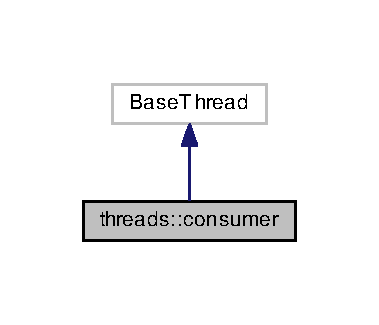
\includegraphics[width=182pt]{dd/dc0/classthreads_1_1consumer__inherit__graph}
\end{center}
\end{figure}


Collaboration diagram for threads\+:\+:consumer\+:\nopagebreak
\begin{figure}[H]
\begin{center}
\leavevmode
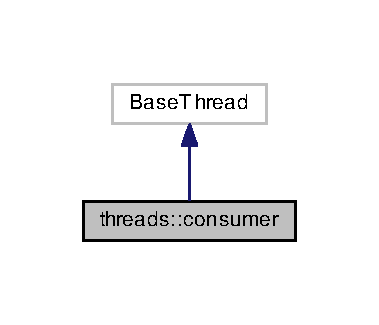
\includegraphics[width=182pt]{d2/de3/classthreads_1_1consumer__coll__graph}
\end{center}
\end{figure}
\subsection*{Public Member Functions}
\begin{DoxyCompactItemize}
\item 
\hyperlink{classthreads_1_1consumer_ae795f2bfd6ded2964f571809e0ea6561}{consumer} ()
\begin{DoxyCompactList}\small\item\em Default constructor. \end{DoxyCompactList}\item 
virtual \hyperlink{classthreads_1_1consumer_aa486915092ce609c11e35b6ac8ae5fe7}{$\sim$consumer} ()
\begin{DoxyCompactList}\small\item\em Destructor. \end{DoxyCompactList}\item 
virtual void \hyperlink{classthreads_1_1consumer_a5c5687cb634bb59115d81e81def30a01}{init} (madara\+::knowledge\+::\+Knowledge\+Base \&knowledge)
\begin{DoxyCompactList}\small\item\em Initializes thread with M\+A\+D\+A\+RA context. \end{DoxyCompactList}\item 
virtual void \hyperlink{classthreads_1_1consumer_aa845379e92c8bb14cd72cb922555c2ec}{run} (void)
\begin{DoxyCompactList}\small\item\em Executes the main thread logic. \end{DoxyCompactList}\end{DoxyCompactItemize}
\subsection*{Private Attributes}
\begin{DoxyCompactItemize}
\item 
madara\+::knowledge\+::\+Knowledge\+Base \hyperlink{classthreads_1_1consumer_ad2ecf700b19fbc6c17f3de8b2e45f39a}{data\+\_\+}
\begin{DoxyCompactList}\small\item\em data plane if we want to access the knowledge base \end{DoxyCompactList}\item 
int \hyperlink{classthreads_1_1consumer_a05d8e8f864be3a9abe4ea6d09dfad46c}{write\+\_\+out\+\_\+interval} = 5
\begin{DoxyCompactList}\small\item\em iterations between writing to file \end{DoxyCompactList}\end{DoxyCompactItemize}


\subsection{Detailed Description}
A custom thread generated by gpc.\+pl. 

Definition at line 18 of file consumer.\+h.



\subsection{Constructor \& Destructor Documentation}
\index{threads\+::consumer@{threads\+::consumer}!consumer@{consumer}}
\index{consumer@{consumer}!threads\+::consumer@{threads\+::consumer}}
\subsubsection[{\texorpdfstring{consumer()}{consumer()}}]{\setlength{\rightskip}{0pt plus 5cm}threads\+::consumer\+::consumer (
\begin{DoxyParamCaption}
{}
\end{DoxyParamCaption}
)}\hypertarget{classthreads_1_1consumer_ae795f2bfd6ded2964f571809e0ea6561}{}\label{classthreads_1_1consumer_ae795f2bfd6ded2964f571809e0ea6561}


Default constructor. 



Definition at line 9 of file consumer.\+cpp.

\index{threads\+::consumer@{threads\+::consumer}!````~consumer@{$\sim$consumer}}
\index{````~consumer@{$\sim$consumer}!threads\+::consumer@{threads\+::consumer}}
\subsubsection[{\texorpdfstring{$\sim$consumer()}{~consumer()}}]{\setlength{\rightskip}{0pt plus 5cm}threads\+::consumer\+::$\sim$consumer (
\begin{DoxyParamCaption}
{}
\end{DoxyParamCaption}
)\hspace{0.3cm}{\ttfamily [virtual]}}\hypertarget{classthreads_1_1consumer_aa486915092ce609c11e35b6ac8ae5fe7}{}\label{classthreads_1_1consumer_aa486915092ce609c11e35b6ac8ae5fe7}


Destructor. 



Definition at line 14 of file consumer.\+cpp.



\subsection{Member Function Documentation}
\index{threads\+::consumer@{threads\+::consumer}!init@{init}}
\index{init@{init}!threads\+::consumer@{threads\+::consumer}}
\subsubsection[{\texorpdfstring{init(madara\+::knowledge\+::\+Knowledge\+Base \&knowledge)}{init(madara::knowledge::KnowledgeBase &knowledge)}}]{\setlength{\rightskip}{0pt plus 5cm}void threads\+::consumer\+::init (
\begin{DoxyParamCaption}
\item[{madara\+::knowledge\+::\+Knowledge\+Base \&}]{knowledge}
\end{DoxyParamCaption}
)\hspace{0.3cm}{\ttfamily [virtual]}}\hypertarget{classthreads_1_1consumer_a5c5687cb634bb59115d81e81def30a01}{}\label{classthreads_1_1consumer_a5c5687cb634bb59115d81e81def30a01}


Initializes thread with M\+A\+D\+A\+RA context. 

Initialization to a knowledge base.


\begin{DoxyParams}{Parameters}
{\em context} & context for querying current program state\\
\hline
\end{DoxyParams}
If you don\textquotesingle{}t actually need access to the knowledge base, just scheduling things in madara\+::threads\+::\+Threader, then you can decide to delete this function or simply do nothing inside of the function. 

Definition at line 25 of file consumer.\+cpp.

\index{threads\+::consumer@{threads\+::consumer}!run@{run}}
\index{run@{run}!threads\+::consumer@{threads\+::consumer}}
\subsubsection[{\texorpdfstring{run(void)}{run(void)}}]{\setlength{\rightskip}{0pt plus 5cm}void threads\+::consumer\+::run (
\begin{DoxyParamCaption}
\item[{void}]{}
\end{DoxyParamCaption}
)\hspace{0.3cm}{\ttfamily [virtual]}}\hypertarget{classthreads_1_1consumer_aa845379e92c8bb14cd72cb922555c2ec}{}\label{classthreads_1_1consumer_aa845379e92c8bb14cd72cb922555c2ec}


Executes the main thread logic. 

Executes the actual thread logic.

Best practice is to simply do one loop iteration. If you want a long running thread that executes something frequently, see the madara\+::threads\+::\+Threader\+::run\+Hz method in your controller. the M\+A\+D\+A\+RA logger is thread-\/safe, fast, and allows for specifying various options like output files and multiple output targets ( e.\+g., std\+::cerr, a system log, and a thread\+\_\+output.\+txt file). You can create your own custom log levels or loggers as well.

Definition at line 38 of file consumer.\+cpp.



\subsection{Member Data Documentation}
\index{threads\+::consumer@{threads\+::consumer}!data\+\_\+@{data\+\_\+}}
\index{data\+\_\+@{data\+\_\+}!threads\+::consumer@{threads\+::consumer}}
\subsubsection[{\texorpdfstring{data\+\_\+}{data_}}]{\setlength{\rightskip}{0pt plus 5cm}madara\+::knowledge\+::\+Knowledge\+Base threads\+::consumer\+::data\+\_\+\hspace{0.3cm}{\ttfamily [private]}}\hypertarget{classthreads_1_1consumer_ad2ecf700b19fbc6c17f3de8b2e45f39a}{}\label{classthreads_1_1consumer_ad2ecf700b19fbc6c17f3de8b2e45f39a}


data plane if we want to access the knowledge base 



Definition at line 44 of file consumer.\+h.

\index{threads\+::consumer@{threads\+::consumer}!write\+\_\+out\+\_\+interval@{write\+\_\+out\+\_\+interval}}
\index{write\+\_\+out\+\_\+interval@{write\+\_\+out\+\_\+interval}!threads\+::consumer@{threads\+::consumer}}
\subsubsection[{\texorpdfstring{write\+\_\+out\+\_\+interval}{write_out_interval}}]{\setlength{\rightskip}{0pt plus 5cm}int threads\+::consumer\+::write\+\_\+out\+\_\+interval = 5\hspace{0.3cm}{\ttfamily [private]}}\hypertarget{classthreads_1_1consumer_a05d8e8f864be3a9abe4ea6d09dfad46c}{}\label{classthreads_1_1consumer_a05d8e8f864be3a9abe4ea6d09dfad46c}


iterations between writing to file 



Definition at line 47 of file consumer.\+h.



The documentation for this class was generated from the following files\+:\begin{DoxyCompactItemize}
\item 
src/threads/\hyperlink{consumer_8h}{consumer.\+h}\item 
src/threads/\hyperlink{consumer_8cpp}{consumer.\+cpp}\end{DoxyCompactItemize}

\hypertarget{classthreads_1_1producer}{}\section{threads\+:\+:producer Class Reference}
\label{classthreads_1_1producer}\index{threads\+::producer@{threads\+::producer}}


A custom thread generated by gpc.\+pl.  




{\ttfamily \#include $<$producer.\+h$>$}



Inheritance diagram for threads\+:\+:producer\+:\nopagebreak
\begin{figure}[H]
\begin{center}
\leavevmode
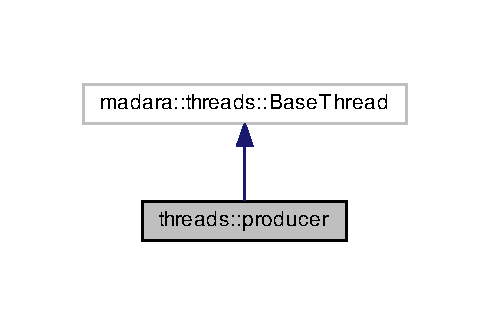
\includegraphics[width=235pt]{dd/d09/classthreads_1_1producer__inherit__graph}
\end{center}
\end{figure}


Collaboration diagram for threads\+:\+:producer\+:\nopagebreak
\begin{figure}[H]
\begin{center}
\leavevmode
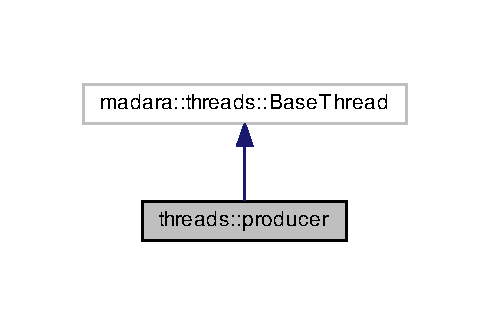
\includegraphics[width=235pt]{d7/de6/classthreads_1_1producer__coll__graph}
\end{center}
\end{figure}
\subsection*{Public Member Functions}
\begin{DoxyCompactItemize}
\item 
\hyperlink{classthreads_1_1producer_a3863c51cfa32b07730d746f414546b37}{producer} ()
\begin{DoxyCompactList}\small\item\em Default constructor. \end{DoxyCompactList}\item 
virtual \hyperlink{classthreads_1_1producer_a2f807ac08bb0a2ad7912ff10cde3c44f}{$\sim$producer} ()
\begin{DoxyCompactList}\small\item\em Destructor. \end{DoxyCompactList}\item 
virtual void \hyperlink{classthreads_1_1producer_a1ec13d5979723407be381557c436fbbf}{init} (madara\+::knowledge\+::\+Knowledge\+Base \&knowledge)
\begin{DoxyCompactList}\small\item\em Initializes thread with M\+A\+D\+A\+RA context. \end{DoxyCompactList}\item 
virtual void \hyperlink{classthreads_1_1producer_aa060b439ac1979c44c8076b59cbe15f8}{run} (void)
\begin{DoxyCompactList}\small\item\em Executes the main thread logic. \end{DoxyCompactList}\end{DoxyCompactItemize}
\subsection*{Protected Attributes}
\begin{DoxyCompactItemize}
\item 
\hyperlink{controller_8cpp_a0584e2a15ee1231298f4501eca6bd1a0}{containers\+::\+Integer} \hyperlink{classthreads_1_1producer_a5ca9ba785a3f49123aea07f960e5497d}{random\+\_\+number}
\end{DoxyCompactItemize}
\subsection*{Private Attributes}
\begin{DoxyCompactItemize}
\item 
madara\+::knowledge\+::\+Knowledge\+Base \hyperlink{classthreads_1_1producer_a9cd75e08b351b2e4e13f3d5b3b4d9e67}{data\+\_\+}
\begin{DoxyCompactList}\small\item\em data plane if we want to access the knowledge base \end{DoxyCompactList}\end{DoxyCompactItemize}


\subsection{Detailed Description}
A custom thread generated by gpc.\+pl. 

Definition at line 18 of file producer.\+h.



\subsection{Constructor \& Destructor Documentation}
\index{threads\+::producer@{threads\+::producer}!producer@{producer}}
\index{producer@{producer}!threads\+::producer@{threads\+::producer}}
\subsubsection[{\texorpdfstring{producer()}{producer()}}]{\setlength{\rightskip}{0pt plus 5cm}threads\+::producer\+::producer (
\begin{DoxyParamCaption}
{}
\end{DoxyParamCaption}
)}\hypertarget{classthreads_1_1producer_a3863c51cfa32b07730d746f414546b37}{}\label{classthreads_1_1producer_a3863c51cfa32b07730d746f414546b37}


Default constructor. 



Definition at line 9 of file producer.\+cpp.

\index{threads\+::producer@{threads\+::producer}!````~producer@{$\sim$producer}}
\index{````~producer@{$\sim$producer}!threads\+::producer@{threads\+::producer}}
\subsubsection[{\texorpdfstring{$\sim$producer()}{~producer()}}]{\setlength{\rightskip}{0pt plus 5cm}threads\+::producer\+::$\sim$producer (
\begin{DoxyParamCaption}
{}
\end{DoxyParamCaption}
)\hspace{0.3cm}{\ttfamily [virtual]}}\hypertarget{classthreads_1_1producer_a2f807ac08bb0a2ad7912ff10cde3c44f}{}\label{classthreads_1_1producer_a2f807ac08bb0a2ad7912ff10cde3c44f}


Destructor. 



Definition at line 14 of file producer.\+cpp.



\subsection{Member Function Documentation}
\index{threads\+::producer@{threads\+::producer}!init@{init}}
\index{init@{init}!threads\+::producer@{threads\+::producer}}
\subsubsection[{\texorpdfstring{init(madara\+::knowledge\+::\+Knowledge\+Base \&knowledge)}{init(madara::knowledge::KnowledgeBase &knowledge)}}]{\setlength{\rightskip}{0pt plus 5cm}void threads\+::producer\+::init (
\begin{DoxyParamCaption}
\item[{madara\+::knowledge\+::\+Knowledge\+Base \&}]{knowledge}
\end{DoxyParamCaption}
)\hspace{0.3cm}{\ttfamily [virtual]}}\hypertarget{classthreads_1_1producer_a1ec13d5979723407be381557c436fbbf}{}\label{classthreads_1_1producer_a1ec13d5979723407be381557c436fbbf}


Initializes thread with M\+A\+D\+A\+RA context. 

Initialization to a knowledge base.


\begin{DoxyParams}{Parameters}
{\em context} & context for querying current program state\\
\hline
\end{DoxyParams}
If you don\textquotesingle{}t actually need access to the knowledge base, just scheduling things in madara\+::threads\+::\+Threader, then you can decide to delete this function or simply do nothing inside of the function. 

Definition at line 25 of file producer.\+cpp.

\index{threads\+::producer@{threads\+::producer}!run@{run}}
\index{run@{run}!threads\+::producer@{threads\+::producer}}
\subsubsection[{\texorpdfstring{run(void)}{run(void)}}]{\setlength{\rightskip}{0pt plus 5cm}void threads\+::producer\+::run (
\begin{DoxyParamCaption}
\item[{void}]{}
\end{DoxyParamCaption}
)\hspace{0.3cm}{\ttfamily [virtual]}}\hypertarget{classthreads_1_1producer_aa060b439ac1979c44c8076b59cbe15f8}{}\label{classthreads_1_1producer_aa060b439ac1979c44c8076b59cbe15f8}


Executes the main thread logic. 

Executes the actual thread logic.

Best practice is to simply do one loop iteration. If you want a long running thread that executes something frequently, see the madara\+::threads\+::\+Threader\+::run\+Hz method in your controller. the M\+A\+D\+A\+RA logger is thread-\/safe, fast, and allows for specifying various options like output files and multiple output targets ( e.\+g., std\+::cerr, a system log, and a thread\+\_\+output.\+txt file). You can create your own custom log levels or loggers as well.

Definition at line 41 of file producer.\+cpp.



\subsection{Member Data Documentation}
\index{threads\+::producer@{threads\+::producer}!data\+\_\+@{data\+\_\+}}
\index{data\+\_\+@{data\+\_\+}!threads\+::producer@{threads\+::producer}}
\subsubsection[{\texorpdfstring{data\+\_\+}{data_}}]{\setlength{\rightskip}{0pt plus 5cm}madara\+::knowledge\+::\+Knowledge\+Base threads\+::producer\+::data\+\_\+\hspace{0.3cm}{\ttfamily [private]}}\hypertarget{classthreads_1_1producer_a9cd75e08b351b2e4e13f3d5b3b4d9e67}{}\label{classthreads_1_1producer_a9cd75e08b351b2e4e13f3d5b3b4d9e67}


data plane if we want to access the knowledge base 



Definition at line 44 of file producer.\+h.

\index{threads\+::producer@{threads\+::producer}!random\+\_\+number@{random\+\_\+number}}
\index{random\+\_\+number@{random\+\_\+number}!threads\+::producer@{threads\+::producer}}
\subsubsection[{\texorpdfstring{random\+\_\+number}{random_number}}]{\setlength{\rightskip}{0pt plus 5cm}{\bf containers\+::\+Integer} threads\+::producer\+::random\+\_\+number\hspace{0.3cm}{\ttfamily [protected]}}\hypertarget{classthreads_1_1producer_a5ca9ba785a3f49123aea07f960e5497d}{}\label{classthreads_1_1producer_a5ca9ba785a3f49123aea07f960e5497d}


Definition at line 48 of file producer.\+h.



The documentation for this class was generated from the following files\+:\begin{DoxyCompactItemize}
\item 
src/threads/\hyperlink{producer_8h}{producer.\+h}\item 
src/threads/\hyperlink{producer_8cpp}{producer.\+cpp}\end{DoxyCompactItemize}

\chapter{File Documentation}
\hypertarget{MainPage_8md}{}\section{docs/\+Main\+Page.md File Reference}
\label{MainPage_8md}\index{docs/\+Main\+Page.\+md@{docs/\+Main\+Page.\+md}}

\hypertarget{controller_8cpp}{}\section{src/controller.cpp File Reference}
\label{controller_8cpp}\index{src/controller.\+cpp@{src/controller.\+cpp}}
{\ttfamily \#include \char`\"{}madara/knowledge/\+Knowledge\+Base.\+h\char`\"{}}\\*
{\ttfamily \#include \char`\"{}madara/threads/\+Threader.\+h\char`\"{}}\\*
{\ttfamily \#include \char`\"{}gams/controllers/\+Base\+Controller.\+h\char`\"{}}\\*
{\ttfamily \#include \char`\"{}gams/loggers/\+Global\+Logger.\+h\char`\"{}}\\*
{\ttfamily \#include \char`\"{}threads/consumer.\+h\char`\"{}}\\*
{\ttfamily \#include \char`\"{}threads/producer.\+h\char`\"{}}\\*
Include dependency graph for controller.\+cpp\+:\nopagebreak
\begin{figure}[H]
\begin{center}
\leavevmode
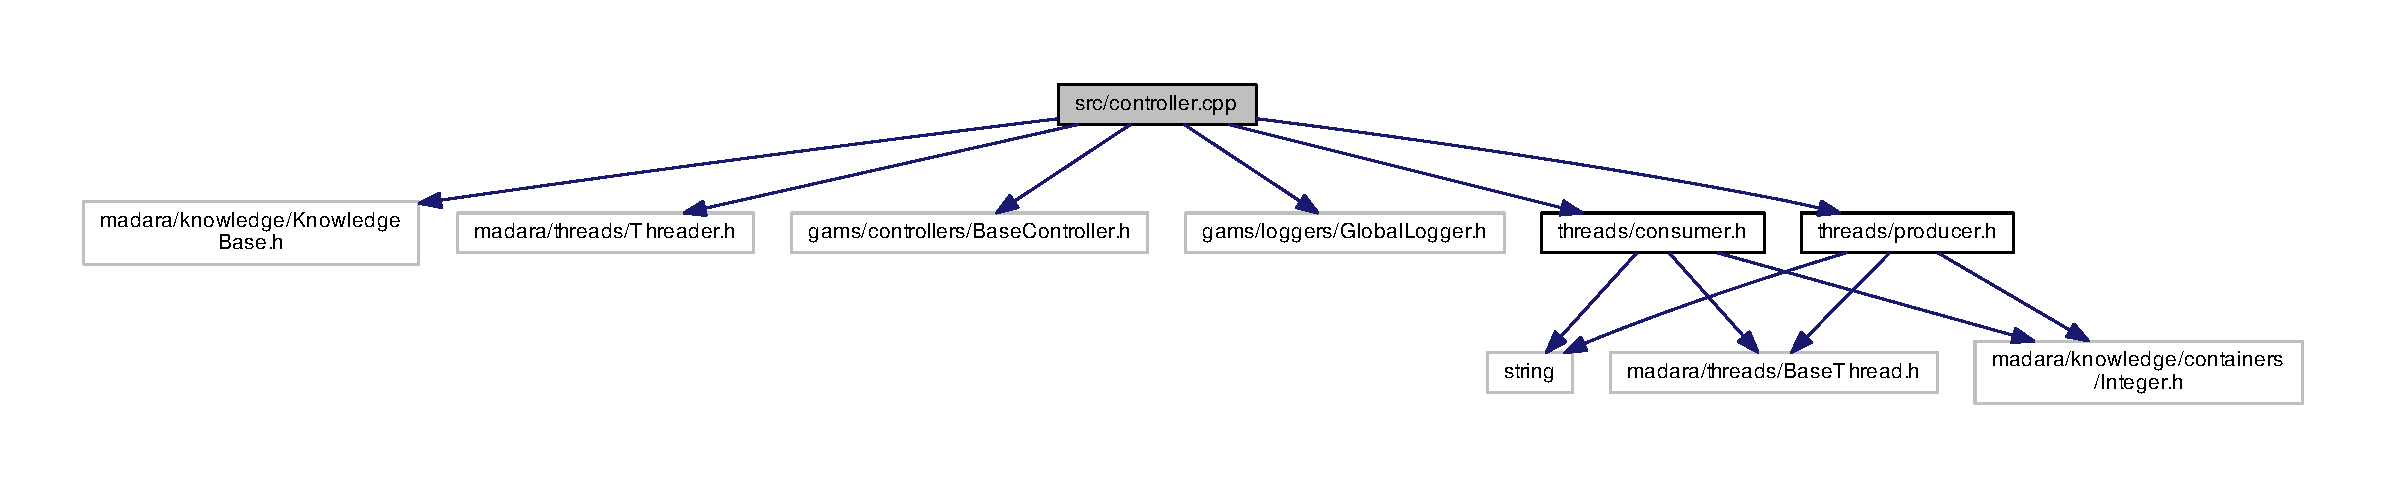
\includegraphics[width=350pt]{d6/d7c/controller_8cpp__incl}
\end{center}
\end{figure}
\subsection*{Typedefs}
\begin{DoxyCompactItemize}
\item 
typedef Record\+::\+Integer \hyperlink{controller_8cpp_a0584e2a15ee1231298f4501eca6bd1a0}{Integer}
\item 
typedef madara\+::knowledge\+::\+Knowledge\+Record \hyperlink{controller_8cpp_abaaae61bd3a8fa0865e1a39d781f1c6a}{Record}
\end{DoxyCompactItemize}
\subsection*{Functions}
\begin{DoxyCompactItemize}
\item 
std\+::string \hyperlink{controller_8cpp_a47d7c31b22b078e7bafd6aa6716af65f}{algorithm} (\char`\"{}debug\char`\"{})
\item 
const std\+::string \hyperlink{controller_8cpp_af6158236a360878159a8e799ee00cf55}{default\+\_\+broadcast} (\char`\"{}192.\+168.\+1.\+255\+:15000\char`\"{})
\item 
const std\+::string \hyperlink{controller_8cpp_aef952081e87739384ba5433cfe4297ae}{default\+\_\+multicast} (\char`\"{}239.\+255.\+0.\+1\+:4150\char`\"{})
\item 
int \hyperlink{controller_8cpp_a4cc3f709921e3e02c780e024add832d3}{gams\+\_\+debug\+\_\+level} (-\/1)
\item 
void \hyperlink{controller_8cpp_a2cfd518572976845680798882117c286}{handle\+\_\+arguments} (int argc, char $\ast$$\ast$argv)
\item 
std\+::string \hyperlink{controller_8cpp_a982f4a462e23a5b6d37f88f16de65200}{host} (\char`\"{}\char`\"{})
\item 
const std\+::string \hyperlink{controller_8cpp_ad130ea69067dbc70ce19d211c78790fb}{K\+N\+O\+W\+L\+E\+D\+G\+E\+\_\+\+B\+A\+S\+E\+\_\+\+P\+L\+A\+T\+F\+O\+R\+M\+\_\+\+K\+EY} (\char`\"{}.platform\char`\"{})
\item 
int \hyperlink{controller_8cpp_a8db2049b790bead0a74fa18c8d9c3248}{madara\+\_\+debug\+\_\+level} (-\/1)
\item 
int \hyperlink{controller_8cpp_a3c04138a5bfe5d72780bb7e82a18e627}{main} (int argc, char $\ast$$\ast$argv)
\item 
\hyperlink{controller_8cpp_a0584e2a15ee1231298f4501eca6bd1a0}{Integer} \hyperlink{controller_8cpp_aee452f6ed6c9d22ef6d6f158593cebab}{num\+\_\+agents} (-\/1)
\item 
std\+::string \hyperlink{controller_8cpp_a6615fcccb5acbeab9bcda3de434f9a06}{platform} (\char`\"{}debug\char`\"{})
\item 
void \hyperlink{controller_8cpp_a5724b5d5bd1fb93f9ae44b8d46b64328}{print\+\_\+usage} (char $\ast$prog\+\_\+name)
\end{DoxyCompactItemize}
\subsection*{Variables}
\begin{DoxyCompactItemize}
\item 
std\+::vector$<$ std\+::string $>$ \hyperlink{controller_8cpp_a7a8184cd712a2cb884729b30455085c2}{accents}
\item 
gams\+::controllers\+::\+Controller\+Settings \hyperlink{controller_8cpp_a870798875407fd034b8a1821a2742010}{controller\+\_\+settings}
\item 
std\+::string \hyperlink{controller_8cpp_abf5d4571e49256d0c9d862dfe4936e55}{file\+\_\+path}
\item 
std\+::string \hyperlink{controller_8cpp_a72c33b609a3d0dd486df35320be2653b}{load\+\_\+transport\+\_\+prefix}
\item 
std\+::string \hyperlink{controller_8cpp_aa29d439d2009d11570344604918bd177}{madara\+\_\+commands} = \char`\"{}\char`\"{}
\item 
bool \hyperlink{controller_8cpp_a7f9805e384e72197c583a2d18af8d7c7}{plat\+\_\+set} = false
\item 
std\+::string \hyperlink{controller_8cpp_ae81934598902069e7e0f607eae169c14}{save\+\_\+transport}
\item 
std\+::string \hyperlink{controller_8cpp_a70f924546b0db8262dae5cc9d9dbed0b}{save\+\_\+transport\+\_\+prefix}
\item 
std\+::string \hyperlink{controller_8cpp_a0d1cbde6bde4c0379bbd29aa8f421737}{save\+\_\+transport\+\_\+text}
\item 
madara\+::transport\+::\+Qo\+S\+Transport\+Settings \hyperlink{controller_8cpp_aeec674db9554192e56960857e748f0ab}{settings}
\end{DoxyCompactItemize}


\subsection{Typedef Documentation}
\index{controller.\+cpp@{controller.\+cpp}!Integer@{Integer}}
\index{Integer@{Integer}!controller.\+cpp@{controller.\+cpp}}
\subsubsection[{\texorpdfstring{Integer}{Integer}}]{\setlength{\rightskip}{0pt plus 5cm}typedef Record\+::\+Integer {\bf Integer}}\hypertarget{controller_8cpp_a0584e2a15ee1231298f4501eca6bd1a0}{}\label{controller_8cpp_a0584e2a15ee1231298f4501eca6bd1a0}


Definition at line 38 of file controller.\+cpp.

\index{controller.\+cpp@{controller.\+cpp}!Record@{Record}}
\index{Record@{Record}!controller.\+cpp@{controller.\+cpp}}
\subsubsection[{\texorpdfstring{Record}{Record}}]{\setlength{\rightskip}{0pt plus 5cm}typedef madara\+::knowledge\+::\+Knowledge\+Record {\bf Record}}\hypertarget{controller_8cpp_abaaae61bd3a8fa0865e1a39d781f1c6a}{}\label{controller_8cpp_abaaae61bd3a8fa0865e1a39d781f1c6a}


Definition at line 37 of file controller.\+cpp.



\subsection{Function Documentation}
\index{controller.\+cpp@{controller.\+cpp}!algorithm@{algorithm}}
\index{algorithm@{algorithm}!controller.\+cpp@{controller.\+cpp}}
\subsubsection[{\texorpdfstring{algorithm(""debug"")}{algorithm("debug")}}]{\setlength{\rightskip}{0pt plus 5cm}std\+::string algorithm (
\begin{DoxyParamCaption}
\item[{\char`\"{}debug\char`\"{}}]{}
\end{DoxyParamCaption}
)}\hypertarget{controller_8cpp_a47d7c31b22b078e7bafd6aa6716af65f}{}\label{controller_8cpp_a47d7c31b22b078e7bafd6aa6716af65f}
\index{controller.\+cpp@{controller.\+cpp}!default\+\_\+broadcast@{default\+\_\+broadcast}}
\index{default\+\_\+broadcast@{default\+\_\+broadcast}!controller.\+cpp@{controller.\+cpp}}
\subsubsection[{\texorpdfstring{default\+\_\+broadcast(""192.\+168.\+1.\+255\+:15000"")}{default_broadcast("192.168.1.255:15000")}}]{\setlength{\rightskip}{0pt plus 5cm}const std\+::string default\+\_\+broadcast (
\begin{DoxyParamCaption}
\item[{\char`\"{}192.\+168.\+1.\+255\+:15000\char`\"{}}]{}
\end{DoxyParamCaption}
)}\hypertarget{controller_8cpp_af6158236a360878159a8e799ee00cf55}{}\label{controller_8cpp_af6158236a360878159a8e799ee00cf55}
\index{controller.\+cpp@{controller.\+cpp}!default\+\_\+multicast@{default\+\_\+multicast}}
\index{default\+\_\+multicast@{default\+\_\+multicast}!controller.\+cpp@{controller.\+cpp}}
\subsubsection[{\texorpdfstring{default\+\_\+multicast(""239.\+255.\+0.\+1\+:4150"")}{default_multicast("239.255.0.1:4150")}}]{\setlength{\rightskip}{0pt plus 5cm}const std\+::string default\+\_\+multicast (
\begin{DoxyParamCaption}
\item[{\char`\"{}239.\+255.\+0.\+1\+:4150\char`\"{}}]{}
\end{DoxyParamCaption}
)}\hypertarget{controller_8cpp_aef952081e87739384ba5433cfe4297ae}{}\label{controller_8cpp_aef952081e87739384ba5433cfe4297ae}
\index{controller.\+cpp@{controller.\+cpp}!gams\+\_\+debug\+\_\+level@{gams\+\_\+debug\+\_\+level}}
\index{gams\+\_\+debug\+\_\+level@{gams\+\_\+debug\+\_\+level}!controller.\+cpp@{controller.\+cpp}}
\subsubsection[{\texorpdfstring{gams\+\_\+debug\+\_\+level(-\/1)}{gams_debug_level(-1)}}]{\setlength{\rightskip}{0pt plus 5cm}int gams\+\_\+debug\+\_\+level (
\begin{DoxyParamCaption}
\item[{-\/}]{1}
\end{DoxyParamCaption}
)}\hypertarget{controller_8cpp_a4cc3f709921e3e02c780e024add832d3}{}\label{controller_8cpp_a4cc3f709921e3e02c780e024add832d3}
\index{controller.\+cpp@{controller.\+cpp}!handle\+\_\+arguments@{handle\+\_\+arguments}}
\index{handle\+\_\+arguments@{handle\+\_\+arguments}!controller.\+cpp@{controller.\+cpp}}
\subsubsection[{\texorpdfstring{handle\+\_\+arguments(int argc, char $\ast$$\ast$argv)}{handle_arguments(int argc, char **argv)}}]{\setlength{\rightskip}{0pt plus 5cm}void handle\+\_\+arguments (
\begin{DoxyParamCaption}
\item[{int}]{argc, }
\item[{char $\ast$$\ast$}]{argv}
\end{DoxyParamCaption}
)}\hypertarget{controller_8cpp_a2cfd518572976845680798882117c286}{}\label{controller_8cpp_a2cfd518572976845680798882117c286}


Definition at line 113 of file controller.\+cpp.

\index{controller.\+cpp@{controller.\+cpp}!host@{host}}
\index{host@{host}!controller.\+cpp@{controller.\+cpp}}
\subsubsection[{\texorpdfstring{host("""")}{host("")}}]{\setlength{\rightskip}{0pt plus 5cm}std\+::string host (
\begin{DoxyParamCaption}
\item[{\char`\"{}\char`\"{}}]{}
\end{DoxyParamCaption}
)}\hypertarget{controller_8cpp_a982f4a462e23a5b6d37f88f16de65200}{}\label{controller_8cpp_a982f4a462e23a5b6d37f88f16de65200}
\index{controller.\+cpp@{controller.\+cpp}!K\+N\+O\+W\+L\+E\+D\+G\+E\+\_\+\+B\+A\+S\+E\+\_\+\+P\+L\+A\+T\+F\+O\+R\+M\+\_\+\+K\+EY@{K\+N\+O\+W\+L\+E\+D\+G\+E\+\_\+\+B\+A\+S\+E\+\_\+\+P\+L\+A\+T\+F\+O\+R\+M\+\_\+\+K\+EY}}
\index{K\+N\+O\+W\+L\+E\+D\+G\+E\+\_\+\+B\+A\+S\+E\+\_\+\+P\+L\+A\+T\+F\+O\+R\+M\+\_\+\+K\+EY@{K\+N\+O\+W\+L\+E\+D\+G\+E\+\_\+\+B\+A\+S\+E\+\_\+\+P\+L\+A\+T\+F\+O\+R\+M\+\_\+\+K\+EY}!controller.\+cpp@{controller.\+cpp}}
\subsubsection[{\texorpdfstring{K\+N\+O\+W\+L\+E\+D\+G\+E\+\_\+\+B\+A\+S\+E\+\_\+\+P\+L\+A\+T\+F\+O\+R\+M\+\_\+\+K\+E\+Y("".\+platform"")}{KNOWLEDGE_BASE_PLATFORM_KEY(".platform")}}]{\setlength{\rightskip}{0pt plus 5cm}const std\+::string K\+N\+O\+W\+L\+E\+D\+G\+E\+\_\+\+B\+A\+S\+E\+\_\+\+P\+L\+A\+T\+F\+O\+R\+M\+\_\+\+K\+EY (
\begin{DoxyParamCaption}
\item[{\char`\"{}.platform\char`\"{}}]{}
\end{DoxyParamCaption}
)}\hypertarget{controller_8cpp_ad130ea69067dbc70ce19d211c78790fb}{}\label{controller_8cpp_ad130ea69067dbc70ce19d211c78790fb}
\index{controller.\+cpp@{controller.\+cpp}!madara\+\_\+debug\+\_\+level@{madara\+\_\+debug\+\_\+level}}
\index{madara\+\_\+debug\+\_\+level@{madara\+\_\+debug\+\_\+level}!controller.\+cpp@{controller.\+cpp}}
\subsubsection[{\texorpdfstring{madara\+\_\+debug\+\_\+level(-\/1)}{madara_debug_level(-1)}}]{\setlength{\rightskip}{0pt plus 5cm}int madara\+\_\+debug\+\_\+level (
\begin{DoxyParamCaption}
\item[{-\/}]{1}
\end{DoxyParamCaption}
)}\hypertarget{controller_8cpp_a8db2049b790bead0a74fa18c8d9c3248}{}\label{controller_8cpp_a8db2049b790bead0a74fa18c8d9c3248}
\index{controller.\+cpp@{controller.\+cpp}!main@{main}}
\index{main@{main}!controller.\+cpp@{controller.\+cpp}}
\subsubsection[{\texorpdfstring{main(int argc, char $\ast$$\ast$argv)}{main(int argc, char **argv)}}]{\setlength{\rightskip}{0pt plus 5cm}int main (
\begin{DoxyParamCaption}
\item[{int}]{argc, }
\item[{char $\ast$$\ast$}]{argv}
\end{DoxyParamCaption}
)}\hypertarget{controller_8cpp_a3c04138a5bfe5d72780bb7e82a18e627}{}\label{controller_8cpp_a3c04138a5bfe5d72780bb7e82a18e627}
W\+A\+R\+N\+I\+NG\+: the following section will be regenerated whenever new threads are added via this tool. So, you can adjust hertz rates and change how the thread is initialized, but the entire section will be regenerated with all threads in the threads directory, whenever you use the new thread option with the gpc.\+pl script.

E\+ND W\+A\+R\+N\+I\+NG

Definition at line 463 of file controller.\+cpp.

\index{controller.\+cpp@{controller.\+cpp}!num\+\_\+agents@{num\+\_\+agents}}
\index{num\+\_\+agents@{num\+\_\+agents}!controller.\+cpp@{controller.\+cpp}}
\subsubsection[{\texorpdfstring{num\+\_\+agents(-\/1)}{num_agents(-1)}}]{\setlength{\rightskip}{0pt plus 5cm}{\bf Integer} num\+\_\+agents (
\begin{DoxyParamCaption}
\item[{-\/}]{1}
\end{DoxyParamCaption}
)}\hypertarget{controller_8cpp_aee452f6ed6c9d22ef6d6f158593cebab}{}\label{controller_8cpp_aee452f6ed6c9d22ef6d6f158593cebab}
\index{controller.\+cpp@{controller.\+cpp}!platform@{platform}}
\index{platform@{platform}!controller.\+cpp@{controller.\+cpp}}
\subsubsection[{\texorpdfstring{platform(""debug"")}{platform("debug")}}]{\setlength{\rightskip}{0pt plus 5cm}std\+::string platform (
\begin{DoxyParamCaption}
\item[{\char`\"{}debug\char`\"{}}]{}
\end{DoxyParamCaption}
)}\hypertarget{controller_8cpp_a6615fcccb5acbeab9bcda3de434f9a06}{}\label{controller_8cpp_a6615fcccb5acbeab9bcda3de434f9a06}
\index{controller.\+cpp@{controller.\+cpp}!print\+\_\+usage@{print\+\_\+usage}}
\index{print\+\_\+usage@{print\+\_\+usage}!controller.\+cpp@{controller.\+cpp}}
\subsubsection[{\texorpdfstring{print\+\_\+usage(char $\ast$prog\+\_\+name)}{print_usage(char *prog_name)}}]{\setlength{\rightskip}{0pt plus 5cm}void print\+\_\+usage (
\begin{DoxyParamCaption}
\item[{char $\ast$}]{prog\+\_\+name}
\end{DoxyParamCaption}
)}\hypertarget{controller_8cpp_a5724b5d5bd1fb93f9ae44b8d46b64328}{}\label{controller_8cpp_a5724b5d5bd1fb93f9ae44b8d46b64328}


Definition at line 68 of file controller.\+cpp.



\subsection{Variable Documentation}
\index{controller.\+cpp@{controller.\+cpp}!accents@{accents}}
\index{accents@{accents}!controller.\+cpp@{controller.\+cpp}}
\subsubsection[{\texorpdfstring{accents}{accents}}]{\setlength{\rightskip}{0pt plus 5cm}std\+::vector$<$std\+::string$>$ accents}\hypertarget{controller_8cpp_a7a8184cd712a2cb884729b30455085c2}{}\label{controller_8cpp_a7a8184cd712a2cb884729b30455085c2}


Definition at line 44 of file controller.\+cpp.

\index{controller.\+cpp@{controller.\+cpp}!controller\+\_\+settings@{controller\+\_\+settings}}
\index{controller\+\_\+settings@{controller\+\_\+settings}!controller.\+cpp@{controller.\+cpp}}
\subsubsection[{\texorpdfstring{controller\+\_\+settings}{controller_settings}}]{\setlength{\rightskip}{0pt plus 5cm}gams\+::controllers\+::\+Controller\+Settings controller\+\_\+settings}\hypertarget{controller_8cpp_a870798875407fd034b8a1821a2742010}{}\label{controller_8cpp_a870798875407fd034b8a1821a2742010}


Definition at line 66 of file controller.\+cpp.

\index{controller.\+cpp@{controller.\+cpp}!file\+\_\+path@{file\+\_\+path}}
\index{file\+\_\+path@{file\+\_\+path}!controller.\+cpp@{controller.\+cpp}}
\subsubsection[{\texorpdfstring{file\+\_\+path}{file_path}}]{\setlength{\rightskip}{0pt plus 5cm}std\+::string file\+\_\+path}\hypertarget{controller_8cpp_abf5d4571e49256d0c9d862dfe4936e55}{}\label{controller_8cpp_abf5d4571e49256d0c9d862dfe4936e55}


Definition at line 57 of file controller.\+cpp.

\index{controller.\+cpp@{controller.\+cpp}!load\+\_\+transport\+\_\+prefix@{load\+\_\+transport\+\_\+prefix}}
\index{load\+\_\+transport\+\_\+prefix@{load\+\_\+transport\+\_\+prefix}!controller.\+cpp@{controller.\+cpp}}
\subsubsection[{\texorpdfstring{load\+\_\+transport\+\_\+prefix}{load_transport_prefix}}]{\setlength{\rightskip}{0pt plus 5cm}std\+::string load\+\_\+transport\+\_\+prefix}\hypertarget{controller_8cpp_a72c33b609a3d0dd486df35320be2653b}{}\label{controller_8cpp_a72c33b609a3d0dd486df35320be2653b}


Definition at line 63 of file controller.\+cpp.

\index{controller.\+cpp@{controller.\+cpp}!madara\+\_\+commands@{madara\+\_\+commands}}
\index{madara\+\_\+commands@{madara\+\_\+commands}!controller.\+cpp@{controller.\+cpp}}
\subsubsection[{\texorpdfstring{madara\+\_\+commands}{madara_commands}}]{\setlength{\rightskip}{0pt plus 5cm}std\+::string madara\+\_\+commands = \char`\"{}\char`\"{}}\hypertarget{controller_8cpp_aa29d439d2009d11570344604918bd177}{}\label{controller_8cpp_aa29d439d2009d11570344604918bd177}


Definition at line 47 of file controller.\+cpp.

\index{controller.\+cpp@{controller.\+cpp}!plat\+\_\+set@{plat\+\_\+set}}
\index{plat\+\_\+set@{plat\+\_\+set}!controller.\+cpp@{controller.\+cpp}}
\subsubsection[{\texorpdfstring{plat\+\_\+set}{plat_set}}]{\setlength{\rightskip}{0pt plus 5cm}bool plat\+\_\+set = false}\hypertarget{controller_8cpp_a7f9805e384e72197c583a2d18af8d7c7}{}\label{controller_8cpp_a7f9805e384e72197c583a2d18af8d7c7}


Definition at line 41 of file controller.\+cpp.

\index{controller.\+cpp@{controller.\+cpp}!save\+\_\+transport@{save\+\_\+transport}}
\index{save\+\_\+transport@{save\+\_\+transport}!controller.\+cpp@{controller.\+cpp}}
\subsubsection[{\texorpdfstring{save\+\_\+transport}{save_transport}}]{\setlength{\rightskip}{0pt plus 5cm}std\+::string save\+\_\+transport}\hypertarget{controller_8cpp_ae81934598902069e7e0f607eae169c14}{}\label{controller_8cpp_ae81934598902069e7e0f607eae169c14}


Definition at line 60 of file controller.\+cpp.

\index{controller.\+cpp@{controller.\+cpp}!save\+\_\+transport\+\_\+prefix@{save\+\_\+transport\+\_\+prefix}}
\index{save\+\_\+transport\+\_\+prefix@{save\+\_\+transport\+\_\+prefix}!controller.\+cpp@{controller.\+cpp}}
\subsubsection[{\texorpdfstring{save\+\_\+transport\+\_\+prefix}{save_transport_prefix}}]{\setlength{\rightskip}{0pt plus 5cm}std\+::string save\+\_\+transport\+\_\+prefix}\hypertarget{controller_8cpp_a70f924546b0db8262dae5cc9d9dbed0b}{}\label{controller_8cpp_a70f924546b0db8262dae5cc9d9dbed0b}


Definition at line 61 of file controller.\+cpp.

\index{controller.\+cpp@{controller.\+cpp}!save\+\_\+transport\+\_\+text@{save\+\_\+transport\+\_\+text}}
\index{save\+\_\+transport\+\_\+text@{save\+\_\+transport\+\_\+text}!controller.\+cpp@{controller.\+cpp}}
\subsubsection[{\texorpdfstring{save\+\_\+transport\+\_\+text}{save_transport_text}}]{\setlength{\rightskip}{0pt plus 5cm}std\+::string save\+\_\+transport\+\_\+text}\hypertarget{controller_8cpp_a0d1cbde6bde4c0379bbd29aa8f421737}{}\label{controller_8cpp_a0d1cbde6bde4c0379bbd29aa8f421737}


Definition at line 62 of file controller.\+cpp.

\index{controller.\+cpp@{controller.\+cpp}!settings@{settings}}
\index{settings@{settings}!controller.\+cpp@{controller.\+cpp}}
\subsubsection[{\texorpdfstring{settings}{settings}}]{\setlength{\rightskip}{0pt plus 5cm}madara\+::transport\+::\+Qo\+S\+Transport\+Settings settings}\hypertarget{controller_8cpp_aeec674db9554192e56960857e748f0ab}{}\label{controller_8cpp_aeec674db9554192e56960857e748f0ab}


Definition at line 33 of file controller.\+cpp.


\hypertarget{Namespaces_8h}{}\section{src/\+Namespaces.h File Reference}
\label{Namespaces_8h}\index{src/\+Namespaces.\+h@{src/\+Namespaces.\+h}}
\subsection*{Namespaces}
\begin{DoxyCompactItemize}
\item 
 \hyperlink{namespacealgorithms}{algorithms}
\begin{DoxyCompactList}\small\item\em Contains algorithms that can be changed at runtime in G\+A\+MS. \end{DoxyCompactList}\item 
 \hyperlink{namespacecontainers}{containers}
\begin{DoxyCompactList}\small\item\em Contains managed C++ containers that map between C++ variables and knowledge variables. \end{DoxyCompactList}\item 
 \hyperlink{namespacefilters}{filters}
\begin{DoxyCompactList}\small\item\em Contains filters that may shape traffic on-\/send or on-\/receive. \end{DoxyCompactList}\item 
 \hyperlink{namespaceplatforms}{platforms}
\begin{DoxyCompactList}\small\item\em Contains platform drivers and platform threads. \end{DoxyCompactList}\item 
 \hyperlink{namespaceplatforms_1_1threads}{platforms\+::threads}
\begin{DoxyCompactList}\small\item\em Contains threads that will be managed by platform drivers. \end{DoxyCompactList}\item 
 \hyperlink{namespacethreads}{threads}
\begin{DoxyCompactList}\small\item\em Contains threads that will be managed by an agent controller. \end{DoxyCompactList}\end{DoxyCompactItemize}


\subsection{Detailed Description}
\begin{DoxyAuthor}{Author}
James Edmondson \href{mailto:jedmondson@gmail.com}{\tt jedmondson@gmail.\+com}
\end{DoxyAuthor}
This file contains namespace documentation. There is no reason to include this file in any project. It is purely for Doxygen documentation. 
\hypertarget{consumer_8cpp}{}\section{src/threads/consumer.cpp File Reference}
\label{consumer_8cpp}\index{src/threads/consumer.\+cpp@{src/threads/consumer.\+cpp}}
{\ttfamily \#include $<$iostream$>$}\\*
{\ttfamily \#include \char`\"{}gams/loggers/\+Global\+Logger.\+h\char`\"{}}\\*
{\ttfamily \#include \char`\"{}consumer.\+h\char`\"{}}\\*
Include dependency graph for consumer.\+cpp\+:\nopagebreak
\begin{figure}[H]
\begin{center}
\leavevmode
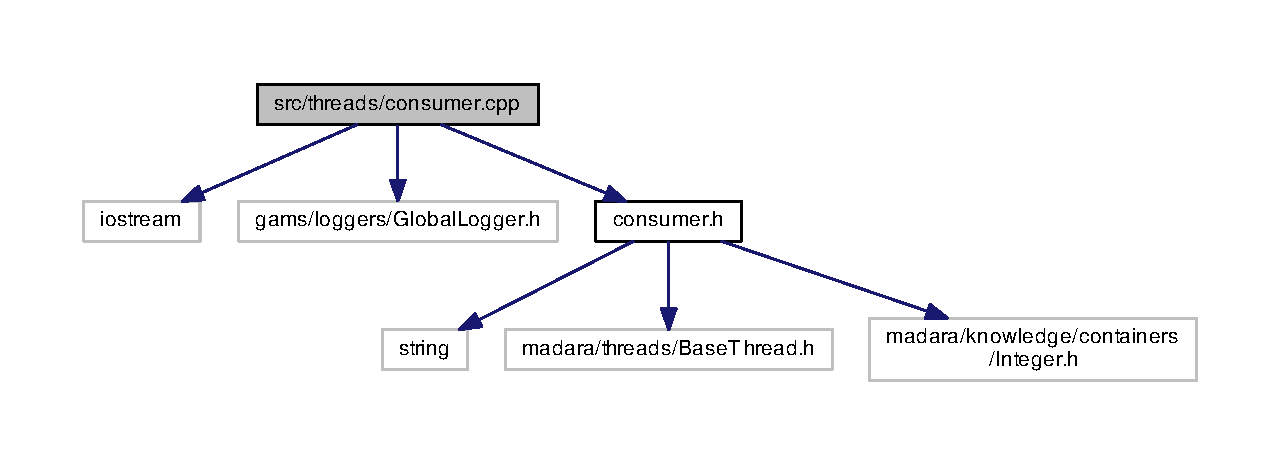
\includegraphics[width=350pt]{de/df6/consumer_8cpp__incl}
\end{center}
\end{figure}

\hypertarget{consumer_8h}{}\section{src/threads/consumer.h File Reference}
\label{consumer_8h}\index{src/threads/consumer.\+h@{src/threads/consumer.\+h}}
{\ttfamily \#include $<$string$>$}\\*
{\ttfamily \#include \char`\"{}madara/threads/\+Base\+Thread.\+h\char`\"{}}\\*
{\ttfamily \#include \char`\"{}madara/knowledge/containers/\+Integer.\+h\char`\"{}}\\*
Include dependency graph for consumer.\+h\+:\nopagebreak
\begin{figure}[H]
\begin{center}
\leavevmode
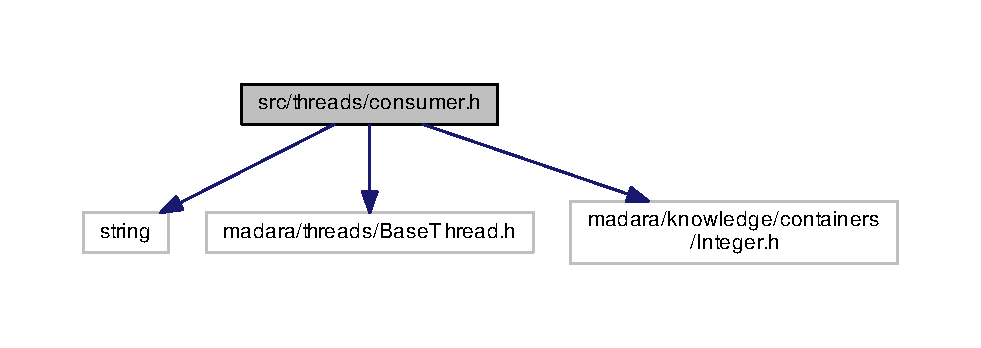
\includegraphics[width=350pt]{da/ddc/consumer_8h__incl}
\end{center}
\end{figure}
This graph shows which files directly or indirectly include this file\+:\nopagebreak
\begin{figure}[H]
\begin{center}
\leavevmode
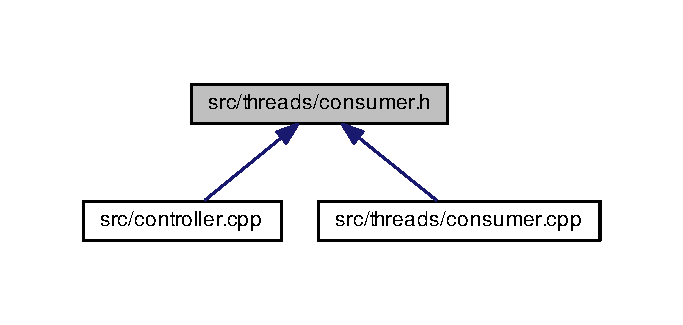
\includegraphics[width=328pt]{d5/d95/consumer_8h__dep__incl}
\end{center}
\end{figure}
\subsection*{Classes}
\begin{DoxyCompactItemize}
\item 
class \hyperlink{classthreads_1_1consumer}{threads\+::consumer}
\begin{DoxyCompactList}\small\item\em A custom thread generated by gpc.\+pl. \end{DoxyCompactList}\end{DoxyCompactItemize}
\subsection*{Namespaces}
\begin{DoxyCompactItemize}
\item 
 \hyperlink{namespacethreads}{threads}
\begin{DoxyCompactList}\small\item\em Contains threads that will be managed by an agent controller. \end{DoxyCompactList}\end{DoxyCompactItemize}

\hypertarget{producer_8cpp}{}\section{src/threads/producer.cpp File Reference}
\label{producer_8cpp}\index{src/threads/producer.\+cpp@{src/threads/producer.\+cpp}}
{\ttfamily \#include $<$iostream$>$}\\*
{\ttfamily \#include \char`\"{}gams/loggers/\+Global\+Logger.\+h\char`\"{}}\\*
{\ttfamily \#include \char`\"{}producer.\+h\char`\"{}}\\*
Include dependency graph for producer.\+cpp\+:\nopagebreak
\begin{figure}[H]
\begin{center}
\leavevmode
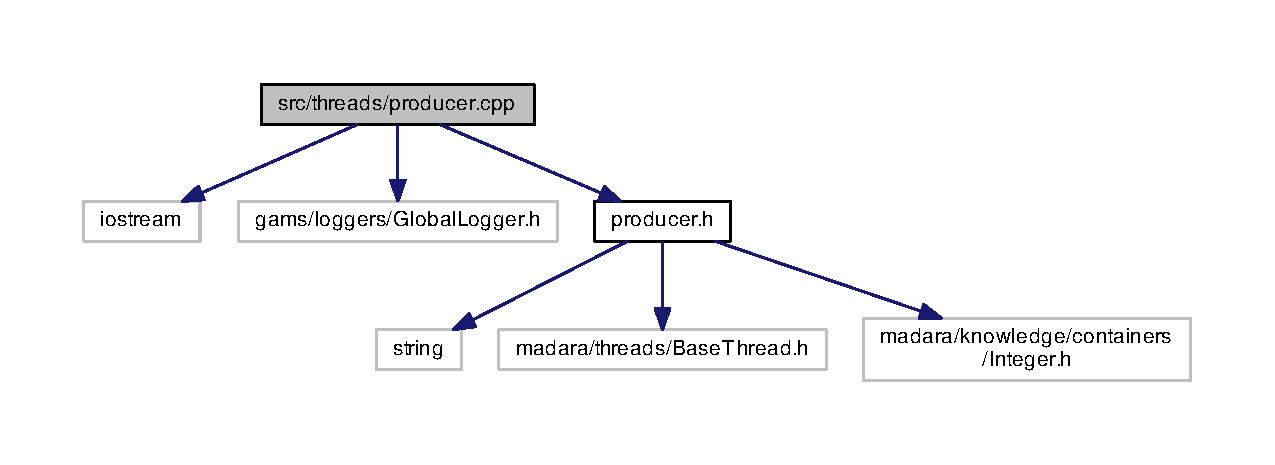
\includegraphics[width=350pt]{d8/db5/producer_8cpp__incl}
\end{center}
\end{figure}

\hypertarget{producer_8h}{}\section{src/threads/producer.h File Reference}
\label{producer_8h}\index{src/threads/producer.\+h@{src/threads/producer.\+h}}
{\ttfamily \#include $<$string$>$}\\*
{\ttfamily \#include \char`\"{}madara/threads/\+Base\+Thread.\+h\char`\"{}}\\*
{\ttfamily \#include \char`\"{}madara/knowledge/containers/\+Integer.\+h\char`\"{}}\\*
Include dependency graph for producer.\+h\+:\nopagebreak
\begin{figure}[H]
\begin{center}
\leavevmode
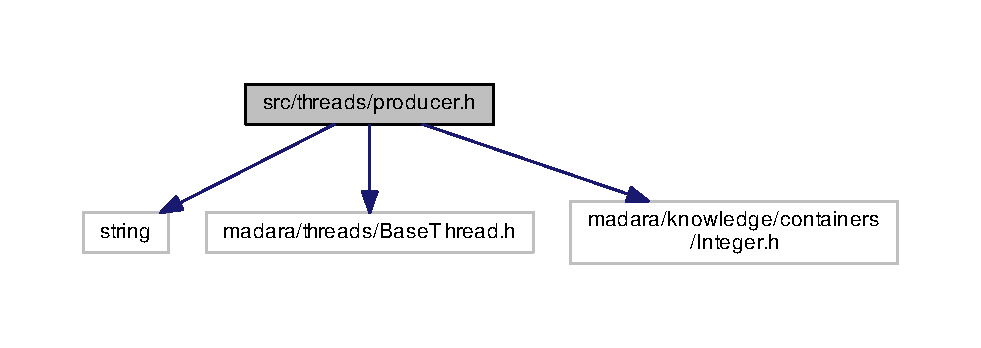
\includegraphics[width=350pt]{d6/d04/producer_8h__incl}
\end{center}
\end{figure}
This graph shows which files directly or indirectly include this file\+:\nopagebreak
\begin{figure}[H]
\begin{center}
\leavevmode
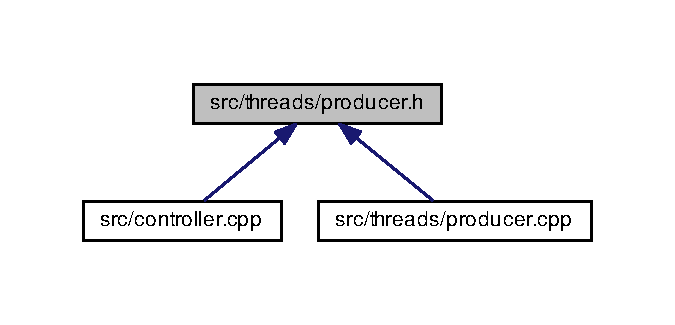
\includegraphics[width=324pt]{d0/d14/producer_8h__dep__incl}
\end{center}
\end{figure}
\subsection*{Classes}
\begin{DoxyCompactItemize}
\item 
class \hyperlink{classthreads_1_1producer}{threads\+::producer}
\begin{DoxyCompactList}\small\item\em A custom thread generated by gpc.\+pl. \end{DoxyCompactList}\end{DoxyCompactItemize}
\subsection*{Namespaces}
\begin{DoxyCompactItemize}
\item 
 \hyperlink{namespacethreads}{threads}
\begin{DoxyCompactList}\small\item\em Contains threads that will be managed by an agent controller. \end{DoxyCompactList}\end{DoxyCompactItemize}

%--- End generated contents ---

% Index
\backmatter
\newpage
\phantomsection
\clearemptydoublepage
\addcontentsline{toc}{chapter}{Index}
\printindex

\end{document}
